\section{Introduction}

With each year new companies jumping into the \emph{IoT} sector and all the major \emph{IT actors} investing and developing products\footnote{https://www.fortunebusinessinsights.com/industry-reports/internet-of-things-iot-market-100307}, as well as telecoms building new infrastructure. The \emph{Internet of Things} has undoubtedly been a subject of hype during the last decade while still maintaining a consistent growth until now. 
Business analysts agree that we should expect to reach at least 40 billion installed \emph{IoT} devices by 2027\footnote{https://www.businessinsider.com/internet-of-things-report}. The \emph{Internet of Things} is used to describe inter-connected devices gathering data without the need of human interaction.
We are, as consumer, already familiar with the traditional \emph{IoT} products we use in our households that allow to connect our light bulbs, our fridge and washing machine, ...
Meanwhile we have less knowledge of the industrial usage of \emph{IoT}, also known as \emph{IIoT}. \emph{IIoT} is one of the fastest growing domain of the market. More and more industries are adopting \emph{IoT}  to consolidate their productions with \emph{real-time monitoring}, predictive maintenance on their assets and products, connecting their supply chains, all of this enabled with the help of network of sensors.
This is applicable in a wide spectrum of domains like \emph{smart farming}, \emph{smart cars}, \emph{smart cities}, \emph{energy managements}, ...

\paragraph{}

The common aspect of all of these applications are that they can communicate wirelessly.
A multitude of telecommunication technologies are used or were created to suit this solution and can be categorized by three different characteristics

\begin{itemize}
    \item Long or Short \emph{range}
    \item High or low \emph{data-rate}
    \item Low or high \emph{power usage} 
\end{itemize}

From these characteristics you can only chose two according to the physical law % TODO Explanation needed
The following graphics\ref{fig:commrangegraph} show a classification of the existing wireless communication used in the \emph{IoT} and mix the three main categories.

\begin{itemize}
    \item \emph{Short-Range wireless communication}
    \item \emph{Cellular communication}
    \item \emph{LPWAN communication} Long range, low power and low data-rate
\end{itemize}

\begin{figure}[H] % TODO More info on axis
\centering
\begin{tikzpicture}
    \draw[->,thick] (-0.1,0)--(12,0) node[right]{Range};
    \draw[->,thick] (0,-0.1)--(0,8) node[above]{Data Rate};
    \node[] at (1, -0.5) {10m};
    \draw[] (1,-0.1)--(1,0.1);
    \node[] at (3, -0.5) {100m};
    \draw[] (3,-0.1)--(3,0.1);
    \node[] at (5, -0.5) {1km};
    \draw[] (5,-0.1)--(5,0.1);
    \node[] at (7, -0.5) {10km};
    \draw[] (7,-0.1)--(7,0.1);
    \node[] at (9, -0.5) {100km};
    \draw[] (9,-0.1)--(9,0.1);

    \node[] at (-1.2, 1) {1 kbit/sec};
    \draw[] (-0.1,1)--(0.1,1);
    \node[] at (-1.2, 3) {1 Mbit/sec};
    \draw[] (-0.1,3)--(0.1,3);
    \node[] at (-1.2, 5) {100 Mbit/sec};
    \draw[] (-0.1,5)--(0.1,5);
    \node[] at (-1.2, 7) {1 Gbit/sec};
    \draw[] (-0.1,7)--(0.1,7);
    
    \node[draw] at (8,1.5) (lora) {LoRa};
    \node[draw] at (9.0,0.8) (sigfox) {SigFox};
    \node[draw] at (7.4,2.2) (nb) {NB-IOT};
    \node[draw,dotted,fit=(lora) (sigfox) (nb), label=above:{LPWAN}] {};

    
    \node[draw] at (2.2,3.5) (bluetooth) {Bluetooth};
    \node[draw] at (2.7,2.5) (zigbee) {ZigBee};
    \node[draw] at (2.0,1.8) (ble) {BLE};
    \node[draw] at (3,5) (wifi) {WiFi};
    \node[draw,dotted,fit=(bluetooth) (zigbee) (ble) (wifi), label=above:{Short-range}] {};

    \node[draw] at (6.8,5) (lte) {LTE};
    \node[draw] at (5.8,6) (5g) {5G};
    \node[draw,dotted,fit=(lte) (5g), label=above:{Cellular}] {};
\end{tikzpicture}
\caption{Comparison of the existing IoT wireless technologies by range and data rate}
\label{fig:commrangegraph}
\end{figure}


This work focus only on \emph{LoRa}, a proprietary chirp spread spectrum modulation technique owned by \emph{Semtech} operating in the sub-GHz unlicensed \emph{ISM} band, that will be explained in more details in section \ref{section:lora}.
The main characteristics of \emph{LoRa} is that it trade throughput for range and low power transmission that as already achieved a record distance of 700km with direct line of sight between the receiver and the transmitter\footnote{https://www.thethingsnetwork.org/article/ground-breaking-world-record-lorawan-packet-received-at-702-km-436-miles-distance}. However this case is not a real world example, we should expect a typical range in urban areas of around \emph{~2-5km} and \emph{15km} in suburban areas\cite{8030482}. Fine tuning the \emph{PHY} settings of the protocol also allow to trade communication distance over throughput and a longer band usage which decrease the number of concurrent motes that can communicate over the band\cite{10.1145/2988287.2989163}.

\emph{LoRa} is often used in conjunction with the \emph{LoRaWAN} a point-to-multipoint protocols. \emph{LoRaWAN} is a ALOHA based\cite{loraalliance:lorawanspecification} network using a star-of-stars topology composed of
wirelessly interconnected \emph{motes} sending data to \emph{gateways} which relay messages to central servers over a Cellular or Ethernet connection as we can see in Figure \ref{fig:startopology}.

\begin{figure}[H]
\begin{subfigure}[b]{.5\textwidth}
    \centering
    \begin{tikzpicture}[auto, thick]
      % Place super peers and connect them
      \foreach \place/\name in {{(0,-1)/a}, {(2,0)/b}, {(2.5, -3)/c}}
        \node[gateways] (\name) at \place {};
      \node[server] (d) at (1.5,-1.5) {};
      %
      \foreach \source/\dest in {a/d, b/d}
        \path[dotted] (\source) edge (\dest);
      \path (c) edge (d); % Non dotted
      %
      % Place normal peers
      \foreach \pos/\i in {above right of/1, right of/2, below right of/3}
        \node[motes, \pos =b ] (b\i) {};
      \foreach \speer/\peer in {b/b1,b/b2,b/b3}
        \path[dotted] (\speer) edge (\peer);
      %
      \foreach \pos/\i in {below left of/1, below of/2, left of/3, above right of/4}
        \node[motes, \pos =a ] (a\i) {};
      \foreach \speer/\peer in {a/a1,a/a2,a/a3,a/a4}
        \path[dotted] (\speer) edge (\peer);
      %
      \path[dotted] (b) edge (a4);
    \end{tikzpicture}
    \caption{Star topology}
    \label{fig:startopology}
\end{subfigure}
\hfill
\begin{subfigure}[b]{.5\textwidth}
    \centering
    \begin{tikzpicture}[auto, thick]
      % Place super peers and connect them
      \foreach \place/\name in {{(0,-1)/a}, {(2,0)/b}, {(2, -3)/c}, {(1,1)/d}, {(1.5, -1.5)/f}}
        \node[motes] (\name) at \place {};
      \foreach \source/\dest in {a/b, a/c, b/c, d/b, f/a, f/b, f/c}
        \path[dotted] (\source) edge (\dest);
      %
      % Place normal peers
      \foreach \pos/\i in {above right of/1, right of/2, below right of/3}
        \node[motes, \pos =b ] (b\i) {};
      \foreach \speer/\peer in {b/b1,b/b2,b/b3}
        \path[dotted] (\speer) edge (\peer);
      %
      \foreach \pos/\i in {above left of/1, left of/2, above of/3}
        \node[motes, \pos =d ] (d\i) {};
      \foreach \speer/\peer in {d/d1,d/d2,d/d3}
        \path[dotted] (\speer) edge (\peer);
      %
      \foreach \pos/\i in {below left of/1, below of/2, left of/3}
        \node[motes, \pos =a ] (a\i) {};
      \foreach \speer/\peer in {a/a1,a/a2,a/a3}
        \path[dotted] (\speer) edge (\peer);
    \end{tikzpicture}
    \caption{Mesh Network Topology}
    \label{fig:meshtopology}
\end{subfigure}
\caption{Different LoRa Network Topologies}
\label{fig:topologies}
\end{figure}




The issue we have is \emph{LoRaWAN} does not scale\cite{10.1145/2988287.2989163}, especially in an urban environment where a lot of motes could overlap. \emph{LoRaWAN} is \emph{ALOHA} based and\emph{CSMA} is not possible because \emph{Channel Activity Detection} only detect the preamble of a communication. This mean a lot of collision can occur during a transmission attempt with a gateway. The \emph{LoRaWAN} protocol state that on collision occur the transmission has to be re-done which lead to a bigger energy consumption as well as occupying the channel even more.
Link quality may also vary some motes far away from the gateway may have issue with doing a correct transmission. Environmental factor like temperature, humidity\cite{evaluation_of_the_reliability_of_lora}, have a lot of influence in the link quality.

Also gateways may not be available everywhere, some use cases may not allow the the installation of gateways, which would imply a power and internet connection, that's the case for pipelines and tunnel, % cite here TODO
where we would prefer to only run devices on batteries.

\begin{figure}[H]
    \centering
    \def\angle{0}
    \def\radius{3}
    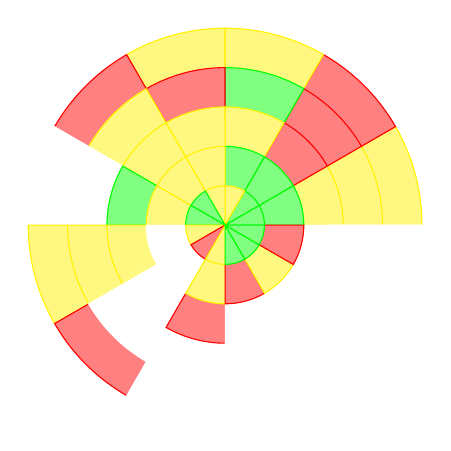
\begin{tikzpicture}[nodes = {font=\sffamily}]
      \foreach \color in {
            yellow,
            red,
            yellow,
            white,
            red,
            yellow,
            white,
            yellow,
            white,
            white,
            red,
            red,
        } {
        \ifx\color\empty\else
            \draw[fill={\color!50},draw={\color}] (0,0) -- (\angle:\radius)
              arc (\angle:\angle+30:\radius) -- cycle;
            \pgfmathparse{\angle+30}
            \xdef\angle{\pgfmathresult}
        \fi
        };
        \xdef\radius{2.5}
        \foreach \color in {
            yellow,
            red,
            yellow,
            yellow,
            red,
            white,
            yellow,
            red,
            white,
            white,
            white,
            white,
        } {
        \ifx\color\empty\else
            \draw[fill={\color!50},draw={\color}] (0,0) -- (\angle:\radius)
              arc (\angle:\angle+30:\radius) -- cycle;
            \pgfmathparse{\angle+30}
            \xdef\angle{\pgfmathresult}
        \fi
        };
        \xdef\radius{2}
        \foreach \color in {
            yellow,
            red,
            green,
            red,
            yellow,
            white,
            yellow,
            white,
            white,
            white,
            white,
            white,
        } {
        \ifx\color\empty\else
            \draw[fill={\color!50},draw={\color}] (0,0) -- (\angle:\radius)
              arc (\angle:\angle+30:\radius) -- cycle;
            \pgfmathparse{\angle+30}
            \xdef\angle{\pgfmathresult}
        \fi
        };
        \xdef\radius{1.5}
        \foreach \color in {
            yellow,
            red,
            yellow,
            yellow,
            yellow,
            green,
            yellow,
            white,
            red,
            white,
            white,
            white,
        } {
        \ifx\color\empty\else
            \draw[fill={\color!50},draw={\color}] (0,0) -- (\angle:\radius)
              arc (\angle:\angle+30:\radius) -- cycle;
            \pgfmathparse{\angle+30}
            \xdef\angle{\pgfmathresult}
        \fi
        };
        \xdef\radius{1}
        \foreach \color in {
            green,
            green,
            green,
            yellow,
            yellow,
            yellow,
            white,
            white,
            yellow,
            red,
            yellow,
            red,
        } {
        \ifx\color\empty\else
            \draw[fill={\color!50},draw={\color}] (0,0) -- (\angle:\radius)
              arc (\angle:\angle+30:\radius) -- cycle;
            \pgfmathparse{\angle+30}
            \xdef\angle{\pgfmathresult}
        \fi
        };
        \xdef\radius{0.5}
        \foreach \color in {
            green,
            green,
            yellow,
            yellow,
            green,
            green,
            yellow,
            red,
            yellow,
            green,
            green,
            green,
        } {
        \ifx\color\empty\else
            \draw[fill={\color!50},draw={\color}] (0,0) -- (\angle:\radius)
              arc (\angle:\angle+30:\radius) -- cycle;
            \pgfmathparse{\angle+30}
            \xdef\angle{\pgfmathresult}
        \fi
        };
    \end{tikzpicture}
\caption{Typical gateway coverage\cite{lorajambalaya}}
\label{fig:coverage}

\begin{tabular}{r@{: }l r@{: }l}
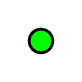
\begin{tikzpicture}\draw[fill=green,line width=1pt]  circle(1ex);\end{tikzpicture} & Good\ Connection & 
\begin{tikzpicture}\draw[fill=yellow,line width=1pt]  circle(1ex);\end{tikzpicture} & Intermediate\ Connection\\
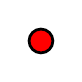
\begin{tikzpicture}\draw[fill=red,line width=1pt]  circle(1ex);\end{tikzpicture} & Bad\ Connection & 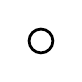
\begin{tikzpicture}\draw[fill=white,line width=1pt]  circle(1ex);\end{tikzpicture} & No\ Connection 
\end{tabular}
\end{figure}




% \begin{tikzpicture}
%     \node[draw] (Application) [abstract, rectangle]{\textbf{Application Layer}};
%     \node[draw] (MAC) [abstract, rectangle, below=0.2cm of Application, text justified]{\textbf{Media Access Control (MAC) Layer}};
%     \node[draw] (Phy) [abstract, rectangle, below=0.2cm of MAC, text justified]{\textbf{Physical (PHY) Layer}};
%     \node[draw] (Rf) [abstract, rectangle, below=0.2cm of Phy, text justified]{\textbf{Radio Frequency (RF) Layer}};
% \end{tikzpicture}

\paragraph{}

That why opting for a multi-hop solution instead of the star network has been proposed and can be an actual good idea to increase the redundancy and the reliability of the lossy network. Gateways are also sensible to power outage and can be a single point a failure of the network while a multi-hop network can adapt to this kind of topological changes. % TODO cite study with the roover water

One of the solution that arised from \emph{IoT} solutions is to use
Time-Slotted Channel Hopping communication to route.


